\title{Concurrency and Parallel Programming \\ Assignment 2}
\author{David van Erkelens and Jelte Fennema \\ Department of Computer Science
    \\ University of Amsterdam} \date{\today}
\documentclass[12pt]{article}
\usepackage{graphicx}
\usepackage{color}
\begin{document}
\maketitle
\section{Notes}
\subsection{One process per core}
As seen in the graphs, the speedup depends on the problem size. When the problem size is small, the speedup is also very small and sometimes even smaller that 1. With a large problem size, the speedup can reach almost 8. This can be explained by the fact that there can be a large communication delay with a small problem size. However, when there is a larger problem size (and thus more calculations), the communication delay will be a smaller percentage of the total executing time.
\subsection{Eight processes per core}
As seen in the graphs, all problem sizes quickly reach their maximum possible speedup. Only the larges problem size doesn't stagnate yet. However, when the problem will be executed on even more cores, this problem size will probably also stagnate, but there's no way to retreive this from the current results.
\clearpage
\section{Graphs}
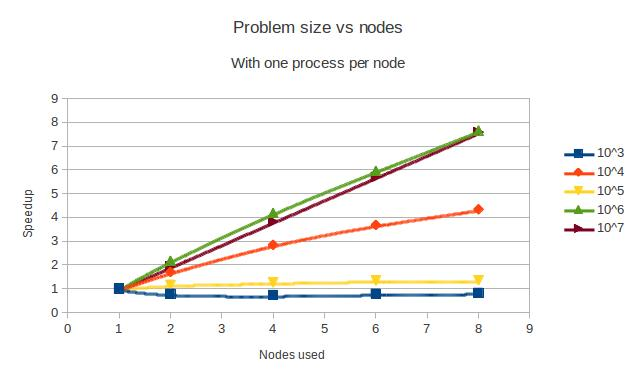
\includegraphics[width=\textwidth]{oneproc.jpg}
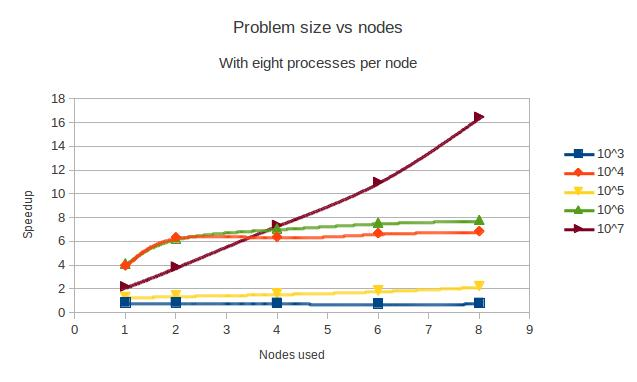
\includegraphics[width=\textwidth]{eightproc.jpg}
\end {document}
